\paraC{Modelling Trust and Risk: $\obeys$, $\MayAccess$ and $\MayAffect$}

The key claim of this paper is that, to reason about the behaviour of
systems in an open world, we need specifications that let us talk
about trust and risk explicitly.  In the rest of this section, we
informally introduce three novel specification language constructs:
$\obeys$ to model trust, and $\MayAccess$ and $\MayAffect$ to model
risk, show how they can be used to specify the purse and escrow
examples, and argue a revised \prg{deal\_version2} method can meet that
specification. \autoref{section:formal} formalises these~ideas.

To model trust, we introduce a special predicate, \obeys, of the
form $o \obeys\ Spec$  which we interpret to mean that
the current object trusts $o$ to adhere to the specification $Spec$.
%
%
Because we generally can't be sure that an object --- especially one
supplied from elsewhere in an open system --- can actually be trusted
to obey a particular specification, our reasoning and specifications
are hypothetical: analysing the same piece of code
under different trust hypotheses --- i.e.\
assuming that particular objects may or may not be trusted to
obey particular specifications.

Thus, {\em if} object \prg{o} can be trusted to obey specification
\prg{Spec}, and \prg{Spec} had a policy describing the behaviour of
some method \prg{m}, then we may expect the method call \prg{o.m(...)}
to behave according to that policy --- otherwise, all bets are off.
% SD I removed the below, as it may be taken to mean that we cannot call the
% method unless we know the object obeys the spec
% This also leads to chains of hypothetical reasoning, as every method
% request on an object needs a case that the receiver obeys the
% specification we hope it does.



% \paraC{Modelling Risk:  $\MayAccess$ and $\MayAffect$}

To model risk, we introduce predicates $\MayAccess$ and $\MayAffect$, which
express whether an object may read or may affect another object or
property. We will write
%
$\MayAffect$\lstinline+(o,p)+
%
to mean that it is possible that some method invocation on \prg{o} would
affect the object or property \lstinline+p+. Similarly, we will write
%
$\MayAccess$\lstinline+(o,p)+
%
to mean that it is possible that the code in object \prg{o} could potentially gain
a capability to access to \lstinline+p+ --- that is, a reference to
\prg{p}.  In
practice, $\MayAccess$\lstinline+(o,p)+ means that \prg{p} is in the
transitive closure of the points-to relation on the heap starting from
\lstinline+o+
including both public and private references.



\paraC{Valid Purse: Specifying \prg{Purse}}


Using $\obeys$, $\MayAccess$, and $\MayAffect$, we write the
 \prg{ValidPurse} specification in Figure~\ref{fig:ValidPurse} that
makes  trust and risk explicit.

\begin{figure*}[hbt]
\begin{lstlisting}[escapechar=&]
specification ValidPurse {
  ghost field balance // Number
  
  abstract predicate CanTrade(p1,p2)

  policy Pol_deposit_1     //   1$^{st}$ case:
      amt$\in \mathbb{N}$
        &\textbf{ \{ res = this.deposit(amt, src) \} }&
      res $\rightarrow$ (
          // TRUST
          CanTrade(this,src)$\PRE{}$  $\wedge$
          // FUNCTIONAL  
          0$\leq$amt$\leq$src.balance$\PRE{}\ \wedge$
          this.balance=this.balance$\PRE$+amt $\wedge$
          src.balance=src.balance$\PRE$-amt  $\wedge$
          //RISK
          $\forall$p.[ p$\obeys$$\pre$ValidPurse $\wedge$ p$\notin\{$this,src$\}\,\rightarrow$
               p.balance=p.balance$\pre$ ]  $\wedge$
          $\forall$o:$\pre$Object. $\forall$p$\obeys$$\pre$ValidPurse.
               [ $\MayAccess$(o,p) $\rightarrow$ $\MayAccess\pre$(o,p) ]   )

  policy Pol_deposit_2     //   2$^{nd}$ case:
      amt$\in \mathbb{N}$
        &\textbf{ \{ res = this.deposit(amt, src) \} }&
       $\neg$res $\rightarrow$ (
          // TRUST and FUNCTIONAL  
          $\neg$[ CanTrade(this,src)$\PRE{}$ $\wedge$ 0$\leq$amt$\leq$src.balance$\PRE{}$ ] $\wedge$
          // RISK
          $\forall$p.[ p$\obeys\PRE{}$ValidPurse$\,\rightarrow\,$ p.balance=p.balance$\pre$ ] $\wedge$
          $\forall$o:$\pre$Object. $\forall$p$\obeys$$\pre$ValidPurse.
               [ $\MayAccess$(o,p) $\rightarrow$ $\MayAccess\pre$(o,p) ]   )
\end{lstlisting}
\vspace*{-7mm}
\caption{\prg{ValidPurse} specification}
\label{fig:ValidPurse}
\end{figure*}
%
\addtocounter{figure}{-1}
%
\begin{figure*}[htb]
\begin{lstlisting}[escapechar=@,firstnumber=32]
  policy Pol_sprout
      true
        @\textbf{ \{ res = this.sprout() \} }@
      // TRUST
      res$\obeys$ ValidPurse $\wedge$  CanTrade(this,res)$\PRE{}$ $\wedge$
      // FUNCTIONAL  
      res.balance=0 $\wedge$
      // RISK
      $\forall$p.[ p$\obeys\PRE$ValidPurse $\rightarrow$
              p.balance=p.balance$\pre$ $\wedge$ res $\neq$ p ]  $\wedge$
      $\forall$o:$\pre$Object. $\forall$p$\obeys$$\pre$ValidPurse.
           [ $\MayAccess$(o,p) $\rightarrow$ $\MayAccess\pre$(o,p) ]    )

  policy Pol_can_trade_constant
       // FUNCTIONAL
       true
        @\textbf{ \{ any\_code \} }@
       $\forall$p:Object.[ CanTrade(p,this) $\longleftrightarrow$ CanTrade$\pre$(p,this) ]

  policy Pol_can_trade_symmetric
         // FUNCTIONAL
         $\forall$p:Object.[ CanTrade(p,this) $\longleftrightarrow$ CanTrade(this,p) ]

  policy Pol_protect_balance
      // RISK
      $\forall$o:Object.[$\MayAffect$(o,this.balance) $\rightarrow$ $\MayAccess$(o,this)]

  policy Trading_is_safe
      // RISK
      $\forall$o:Object.[ CanTrade(o,this) $\rightarrow$  o $\obeys$ ValidPurse ]

}
\end{lstlisting}
\vspace*{-7mm}
\caption{\prg{ValidPurse} specification (contd.)}
\end{figure*}
% SD removed as not necessary to have
% abstract predicate CanTrade(prs1,prs2) is reflexive

%james hates the bullets
%\newcommand{\sophiabullet}{$\bullet$~}
\newcommand{\sophiabullet}{}

\prg{\tobym{ValidPurse}} consists of five policies. % consider the policies in turn.
%The cases
\sophiabullet \prg{Pol\_deposit\_1}  and \sophiabullet \prg{Pol\_deposit\_2} taken together  distinguish between
a successful and an unsuccessful deposit, signalled by
returning \prg{true} or \prg{false} respectively. In the first case, i.e. \prg{Pol\_deposit\_1}
where the result is \prg{true},
argument \prg{src}  must have been
a valid purse
%
(\lstinline+src $\obeys$ ValidPurse+)
%
which can trade with the receiver,
 and \prg{src} must have sufficient balance. In the second case, i.e. \prg{Pol\_deposit\_2}
where the result is \prg{false},
 either \prg{src} was not a valid purse,
or would not trade with the receiver, or had insufficient
funds.
To quote Miller et al.~\cite{ELang}:
``\textit{A reported successful deposit can be trusted as much as one
  trusts the purse one is depositing into}''.


The last two lines in the postcondition of \prg{Pol\_deposit\_1} and
\prg{Pol\_deposit\_2} provide framing conditions.  In the first case,
the transaction will happen, but all other purses will be unmodified
(line 14 in figure \ref{fig:ValidPurse}) , whereas in the second case
no purses will be modified (line 24 in figure \ref{fig:ValidPurse}).
Another framing condition, appears on lines 15, 25 and 36 of figure
\ref{fig:ValidPurse}, and requires that the methods do not leak access
to \jnCUT{(the internals of)} any \prg{ValidPurse} object. In other
words, if \textit{after} the method call, a pre-existing \prg{o} has
access to a \prg{ValidPurse} object \prg{p}, then \prg{o} already had
access to a \prg{p} \textit{before} the call.

% SD I chopped the below, as we talk abpout it again later on
% The \prg{ValidPurse} specification
%uses \obeys\ clauses to reason
%about trust explicitly.  For the reasons described above,
%\prg{ValidPurse} cannot make absolute statements about trust, but can
%support relative, hypothetical statements.
%%
%Consider the request\\ % a deposit request such as
%%
%\SP  \lstinline+res=dest.deposit(amt, src)+\\
%%
%If the destination purse accepts the deposit, then   % can deduce
%we would like to deduce that it has been   able to retrieve the funds
%from the source purse,
%% Ideally, we would like to
%% So, we would like to
%and so assert the {\em absolute} statement that \\
%%
%\SP   \lstinline+res $\rightarrow$  src $\obeys$ ValidPurse+\\
%%
%Unfortunately, the \lstinline+ValidPurse+ specification % as a whole
%only
%applies if the receiver \lstinline+dest+ is trustworthy: we can get
%only as far as the % relative
%{\em conditional} conclusion\\
%%
%\SP  \lstinline+res $\wedge$ dest$\obeys$ValidPurse $\rightarrow$ src$\obeys$ValidPurse+\\
%%
%meaning that, if the \prg{deposit} method returns true, then we can
%trust \prg{src} if we were willing to trust \prg{dest}.
%%SD I trimmed the below -- too many intermediate steps
%%we trust \prg{src} only inasmuch as we trust \prg{dest}.
%%In fact, even this relative conclusion too strong, because the
%%reasoning must be hypothetical: it only applies
%%when a \prg{deposit} request is actually successful (``at runtime''). The
%%best we can conclude is
%%%
%%``\lstinline+res $\rightarrow$ dest $\obeys$ ValidPurse $\rightarrow$ src $\obeys$ ValidPurse+'',
%%%
%%meaning that, if the \prg{deposit} method returns true, then we can
%%trust \prg{src} if we were willing to trust \prg{dest}.
%\noindent So, if an amount is deposited successfully into a
%trustworthy destination \prg{ValidPurse}, that purse vouches that the
%\prg{src} is itself trustworthy.
%% This is essentially what it means to
%% accept a trustworthy deposit, and accepting trustworthy deposits is
%% key to being a trustworthy purse ---




% The remaining policies appear on the continuation Figure: \\

\sophiabullet
\prg{Pol\_sprout} % , the third policy,
promises that the result is a
trusted purse that can trade with the receiver, %change
no other valid
purse's balance is affected, and % that
references % to  valid purses
have not been leaked.


\sophiabullet \prg{Pol\_can\_trade\_constant} guarantees that
whether or not two purses can trade with each other can \textit{never}
change, no matter what code is run.  This is another key ingredient of
our approach: we can require that our code must preserve
properties in the face of unknown code.

\sophiabullet
%
% The fifth policy,
\prg{Pol\_protect\_balance}
% delimits the risk involved with the purses. This policy
guarantees that
 a valid purse \lstinline+p+'s balance can only be changed:
--- \lstinline+$\MayAffect$(o,p.balance)+ ---
by an object \lstinline{o}
that may access that purse:
\lstinline+$\MayAccess$(o,p)+.


Finally, the abstract predicate \prg{CanTrade} holds when two
\prg{Purse}s can trade with each other.  \prg{CanTrade} must be
reflexive, but does not require that its arguments have the same
class. It guarantees that \prg{deposit} can transfer resources from one purse
to another. This could involve a clearing house, interbank exchange,
or other mechanisms % in fact require both purses to be the same class, as an
abstract
predicates can be implemented in different ways.

%  I chpped the below, as we will say it later
% This purse specification is designed to support secure
%\textit{one-way} payments.  To make a payment, the payer will
%typically make a new, empty, temporary purse from one of their
%existing purses via \lstinline+sprout+, and deposit only enough funds
%for the payment into the temporary purse.  The payer then passes the
%temporary purse to the payee, who then empties it back into their
%primary purse.  This allows two \textit{mutually untrusting}
%components to transfer funds, provided that they both trust
%purses involved. Assuming the payer has a \lstinline+payerMainPurse+
%account, and the payee has a \lstinline+payeeMainPurse+ account, then
%the transaction may take place as follows:
%
%\label{s-payment}
%\begin{lstlisting}
%    //payer creates temp purse
%    def tempPurse = payerMainPurse.sprout
%    tempPurse.deposit(100, payerMainPurse)
%    //payer passes tempPurse to payee
%    payee.acceptPayment(100, tempPurse)
%    //payee
%    payeeMainPurse.deposit(100, tempPurse)
%\end{lstlisting}
%
%It is important for the wider system that the \lstinline+deposit+
%method will return true only if both purses actually can trade with
%each other, and that the source purse has sufficient funds ---
%otherwise the \lstinline+deposit+ must return false.
%This turns out to be a
% key trust property of the
%\prg{ValidPurse} specification: if a request like
%%
%\lstinline+res=dest.deposit(0, src)+
%%
%returns true, the \prg{dest} purse can vounch that the \prg{src} purse
%can be trusted.  To see how this could work, imagine each purse
%represents a bank account: a transfer validates the source account
%because the destination account's bank has been able to access the
%funds.  This holds true even though there may many different families
%of purses representing different kinds of resouces in the system, and
%many alternative implementations. In an open system, we cannot expect
%a central authority to know which are trustworthy and which are not.

\scd{The use of assertions about the pre-state in methods' postconditions increases the expressive power of our specifications. For example, consider:\\
\noindent (A)~\prg{amt} $\in \mathbb{N}$ {\bf\ttfamily\small {\{res=this.deposit(amt,src)\}}} \prg{res} $\rightarrow$
    \prg{scr} $\obeys\PRE$\prg{ValidPurse}\\
This allows us to deduce properties about the pre-state by  observing the result of the method call.
Such a specification cannot be easily translated into one which does not make use of this facility, as in:\\
\noindent (B)~\prg{scr} $\obeys$\prg{ValidPurse} $\wedge$ \prg{amt} $\in \mathbb{N}$ {\bf\ttfamily\small{\{res=this.deposit(amt,src)\}}} \prg{res} \\
(B) differs from (A) in that (B) requires us to establish that  \prg{scr} $\obeys$\prg{ValidPurse} before making the call, while
(A) does not.
}



\paraC{Establishing Mutual Trust}
\label{section:mutualTrust}
An escrow must build a two-way, trusted transfer by combining one-way
transfers.
%  The key to a successful escrow is establishing just enough
% mutual trust for just long enough for the two parties to be able to
% complete the transaction.
From \prg{Pol\_deposit\_1} we obtain that %  We have argued that
the call
%
\mbox{\lstinline+res1=dest.deposit(amt, src)+}
%
lets us conclude
%
\mbox{\lstinline+res1 $\wedge$ dest$\obeys$ValidPurse $\rightarrow$ src$\obeys$ValidPurse+}.
This trust
is
just one way: from the destination to the source purse.
% Our earlier informal work
%\cite{capeFTfJP14} offers  a key insight: we can
We can establish mutual trust between two purses by then attempting to
perform a second
deposit \emph{in the reverse direction} from destination to source:
%
\mbox{\lstinline+res2=src.deposit(amt, dest)+}
%
\noindent which in turn gives % lets us conclude that
%
\mbox{\lstinline+res2 $\wedge$ src$\obeys$ValidPurse $\rightarrow$ dest$\obeys$ValidPurse+}.
%
\noindent Reasoning conditionally,
  on a path where \lstinline+res1 $\wedge$ res2+ are
  true,
we can then establish mutual trust:\\
$ \SP \SP \SP \SP \SP\SP   $ \mbox{\lstinline+dest $\obeys$ ValidPurse\   $\longleftrightarrow$ \   src $\obeys$ ValidPurse+}
%
\\  \kjx{We establish this
formally in \autoref{section:formalPROOF},
having only argued informally earlier
\cite{swapsiesOnTheInternet2015,capeFTfJP14}.}

As with much of our reasoning, this is both conditional and
hypothetical: at a particular code point, when two \prg{deposit}
requests have succeeded (or rather, that they have both
\textit{reported} success) then we can conclude that either both are
trust worthy, or both are untrustworthy: we have only {\em hypothetical}
knowledge of the $\obeys$ predicate.


\paraC{Escrow with Explicit Mutual Trust}
\label{sec:mutual-trust}

\forget{
%SD I made a shorter version
\begin{figure}[htb]
\begin{lstlisting}
method dealV2(  ) // returns Boolean
{
  //setup and validate Money purses
  escrowMoney = sellerMoney.sprout
  res=escrowMoney.deposit(0, sellerMoney)
  if (!res) then {return false}
  res = buyerMoney.deposit(0, escrowMoney)
  if (!res) then {return false}
  res = escrowMoney.deposit(0, buyerMoney)
  if (!res) then {return false}

  //setup and validate Goods purses
  escrowGoods = buyerGoods.sprout
  res=escrowGoods.deposit(0, buyerGoods)
  if (!res) then {return false}
  res = sellerGoods.deposit(0, escrowGoods)
  if (!res) then {return false}
  res = escrowGoods.deposit(0, sellerGoods)
  if (!res) then {return false}

  res = escrowMoney.deposit(price, buyerMoney)
  if (!res) then {return false}
  res = escrowGoods.deposit(amt, sellerGoods)
  if (!res) then {
    buyerMoney.deposit(price, escrowMoney)
    return false}

  sellerMoney.deposit(price, escrowMoney)
  buyerGoods.deposit(amt, escrowGoods)

  return true
}
\end{lstlisting}
\vspace*{-7mm}
\caption{Second Attempt at Escrow \preg{deal} method}
\label{fig:DealV2}
\end{figure}
}

\begin{figure}[htb]
\begin{lstlisting}
method deal_version2(  ) // returns Boolean
{
  // setup and validate Money purses
  escrowMoney = sellerMoney.sprout
  res=escrowMoney.deposit(0, sellerMoney)
  if (!res) then {return false}
  res = buyerMoney.deposit(0, escrowMoney)
  if (!res) then {return false}
  res = escrowMoney.deposit(0, buyerMoney)
  if (!res) then {return false}

  // setup and validate Goods purses
  // similar to lines 4-10 from above, but for Goods

  // make the transaction
  // as in lines 8-29 from Fig.1
}
\end{lstlisting}
\vspace*{-7mm}
\caption{Revised \prg{deal\_version2} method}
\label{fig:DealV2}
\end{figure}


Two way deposit calls are sufficient to establish mutual trust,
but come with risks.
For example, as part of
validating that a buyer's  % money
purse %  mutually trusts
the seller's
% money
purse, we must  pass the buyer's purse
as an argument in a
\prg{deposit} call to the seller's % money
purse, e.g.\\
%
~ \SP \lstinline+sellerMoney.deposit(0, buyerMoney)+\\
%
\noindent
If the seller's purse is not in fact trustworthy, then it can take this
opportunity to steal all the money in the buyer's purse before the
transaction officially starts, even if the \prg{amt} that is supposed
to be deposited is \prg{0}.

We can minimise this risk by careful use of escrow purses. Rather than
mutually validating buyers and sellers directly, we can create an escrow
purse on the destination side of the transaction (the seller's money
and the buyer's goods) and then mutually validate the buyer's and
sellers actual purses against the escrow --- resulting in a chain of
mutual trust between the destination purse and the escrow purse, and
the escrow purse and the source purse. This allows us to hypothesise
that the source and destination purses are mutually trusting before we
start on the transaction proper.




The resulting escrow method is in
Figure~\ref{fig:DealV2}. Line~4 creates a \prg{escrowMoney}
purse and then lines~5--10 hypothetically establish mutual trust
between the \prg{escrowMoney}, \prg{sellerMoney}, and \prg{buyerMoney}
purses.   The \prg{sellerMoney} purse doesn't need to validate
\prg{escrowMoney}  explicitly
(\prg{sellerMoney.deposit(0,escrowMoney)}) because the \prg{sprout}
method specification says sprouted purses can trusted as much as their
parent purses.
%
\begin{figure}[h]
  \centering
  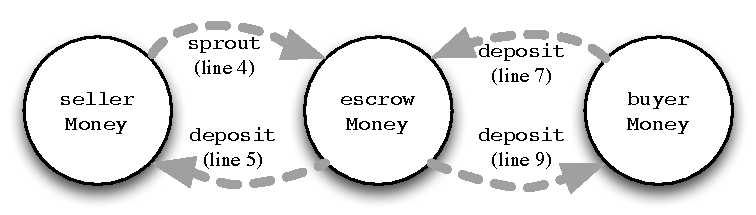
\includegraphics[scale=0.8]{mutual-trust-landscape.pdf}
  \vspace*{-4mm}
  \caption{Establishing Mutual Trust. Dashed arrows show purse validation.}
  \label{fig:mutual-trust}
\end{figure}
%
\noindent (Figure~\ref{fig:mutual-trust} illustrates the trust
relationships.)
If any of these
\prg{deposit} request fail, we abort.
% Lines~13--19 do
Afterwards we do exactly the same, but for goods purses rather than
money purses.  Finally, % lines~21--31
we carry out the escrow exchange
itself, in exactly the same manner as lines~8--29 of the first % escrow
implementation
in Figure~\ref{fig:DealV1}.


\paraC{Specifying the Mutual Trust Escrow}
\label{sec:VaildEscrow}


\begin{figure*}[hbt]
\begin{lstlisting}[escapechar=@]
specification ValidEscrow {
   fields sellerMoney, sellerGoods, buyerMoney, buyerGoods
   fields price, amt   // $\mathbb{N}$

 policy Pol_deal
  price,amt$\in \mathbb{N}$ $\wedge$ price,amt>0
      @\textbf{  \{  this.deal( \ ) \} }@
  res $\wedge$ BadPPrs=$\emptyset$  $\rightarrow$ (      //   1$^{st}$ case:
    CanTrade(buyerMoney,sellerMoney) $\wedge$
    CanTrade(buyerGoods,sellerGoods) $\wedge$
    buyerMoney.balance=buyerMoney.balance$\pre$-price $\wedge$
    sellerMoney.balance=sellerMoney.balance$\pre$+price$\wedge$
    buyerGoods.balance=buyerGoods.balance$\pre$+amt $\wedge$
    sellerGoods.balance=sellerGoods.balance$\pre$-amt $\wedge$
    $\forall$p:$\pre$OthrPrs. p.balance=p.balance.$\pre$  $\wedge$
    $\forall$o:$\pre$Object,p:$\pre$GoodPrs.
         ($\MayAccess$(o,p) $\rightarrow \MayAccess$(o,p)$\pre$) )
  $\wedge$
  $\neg$res $\wedge$ BadPPrs=$\emptyset$   $\rightarrow$ (   //   2$^{nd}$ case:
    $\neg$( CanTrade(buyerMoney,sellerMoney) $\wedge$
         CanTrade(buyerGoods,sellerGoods) $\wedge$
         buyerMoney.balance$\pre  \geq$ price $\wedge$
         sellerGoods.balance$\pre \geq$ amt ) $\wedge$
    $\forall$p:$\pre$GoodPrs. p.balance=p.balance.$\pre$   $\wedge$
    $\forall$o:$\pre$Object,p:$\pre$GoodPrs.
          ($\MayAccess$(o,p) $\rightarrow \MayAccess$(o,p)$\pre$)   )
  $\wedge$
  $\neg$res $\wedge$ BadPPrs$\neq$$\emptyset$  $\rightarrow$  (  //   3$^{rd}$ case:
    $\forall$p:$\pre$GoodPrs. (p.balance=p.balance.$\pre$ $\vee$
           $\exists$ bp$\in$BadPPrs$\pre.\, \MayAccess$(bp,p)$\pre$)  $\wedge$
    $\forall$o:$\pre$Object,p:$\pre$GoodPrs.( $\MayAccess$(o,p) $\rightarrow$
         ($\MayAccess$(o,p)$\pre$ $\vee \exists$b$\in$BadPPrs$\pre$.$\MayAccess$(b,p)$\pre$)) )
  $\wedge$
  res $\wedge$ BadPPrs$\neq\emptyset$   $\rightarrow$  (    //   4$^{th}$ case:
    buyerMoney$\obeys$ValidPurse $\longleftrightarrow$ sellerMoney$\obeys$ValidPurse  $\wedge$
    buyerGoods$\obeys$ValidPurse $\longleftrightarrow$ sellerGoods$\obeys$ValidPurse  $\wedge$
    $\forall$p:$\pre$OthrPrs. (p.balance=p.balance.$\pre$ $\vee$
        $\exists$bp$\in$ BadPPrs$\pre.\, \MayAccess$(bp,p)$\pre$)  $\wedge$
    $\forall$o:$\pre$Object,p:$\pre$GoodPrs. ($\MayAccess$(o,p)$\rightarrow$
       ($\MayAccess$(o,p)$\pre$$\vee \exists$b$\in$BadPPrs$\pre$.$\MayAccess$(b,p)$\pre$)) )
}
\end{lstlisting}
\vspace*{-7mm}
\caption{\prg{ValidEscrow} specification}
\label{fig:ValidEscrow}
\end{figure*}


%\forget{
%% SD made a shorter version
%\begin{figure*}[hbt]
%\begin{lstlisting}[escapechar=@]
%specification ValidEscrow {
%   fields sellerMoney, sellerGoods, buyerMoney, buyerGoods
%   fields price, amt   // $\mathbb{N}$
%
% policy Pol_deal_1    //   1$^{st}$ case:
%   price,amt$\in \mathbb{N}$ $\wedge$ price,amt>0
%      @\textbf{  \{  this.deal( \ ) \} }@
%    res $\wedge$ BadPPrs=$\emptyset$  $\rightarrow$ (
%      // FUNCTIONAL SPECIFICATION
%     CanTrade(buyerMoney,sellerMoney) $\wedge$                            CanTrade(buyerGoods,sellerGoods) $\wedge$
%      buyerMoney.balance=buyerMoney.balance$\pre$-price $\wedge$              sellerMoney.balance=sellerMoney.balance$\pre$+price$\wedge$
%      buyerGoods.balance=buyerGoods.balance$\pre$+amt $\wedge$                sellerGoods.balance=sellerGoods.balance$\pre$-amt $\wedge$
%      // RISK
%      $\forall$p:$\pre$OthrPrs. p.balance=p.balance.$\pre$  $\wedge$
%      $\forall$o:$\pre$Object,p:$\pre$GoodPrs.                                     $\MayAccess$(o,p) $\rightarrow \MayAccess$(o,p)$\pre$)
%
% policy Pol_deal_2    //   2$^{nd}$ case:
%    price,amt$\in \mathbb{N}$ $\wedge$ price,amt>0
%       @\textbf{  \{  this.deal( \ ) \} }@
%    $\neg$res $\wedge$ BadPPrs=$\emptyset$  $\rightarrow$ (
%       // FUNCTIONAL SPECIFICATION
%       $\neg$( CanTrade(buyerMoney,sellerMoney) $\wedge$                          CanTrade(buyerGoods,sellerGoods) $\wedge$
%            buyerMoney.balance$\pre  \geq$ price $\wedge$                            sellerGoods.balance$\pre \geq$ amt ) $\wedge$
%      // RISK
%      $\forall$p:$\pre$GoodPrs. p.balance=p.balance.$\pre$   $\wedge$
%      $\forall$o:$\pre$Object,p:$\pre$GoodPrs.                                        $\MayAccess$(o,p) $\rightarrow \MayAccess$(o,p)$\pre$  )
%\end{lstlisting}
%\vspace*{-7mm}
%\caption{\prg{ValidEscrow} specification}
%\label{fig:ValidEscrow}
%\end{figure*}
%%
%\addtocounter{figure}{-1}
%%
%\begin{figure*}[htb]
%\begin{lstlisting}[escapechar=@,firstnumber=38]
% policy Pol_deal_3    //   3$^{rd}$ case:
%    price,amt$\in \mathbb{N}$ $\wedge$ price,amt>0
%       @\textbf{  \{  this.deal( \ ) \} }@
%    $\neg$res $\wedge$ BadPPrs$\neq$$\emptyset$  $\rightarrow$  (
%       //RISK
%       $\forall$p:$\pre$GoodPrs. ( p.balance=p.balance.$\pre$ $\vee$                   $\exists$ bp$\in$BadPPrs$\pre.\, \MayAccess$(bp,p)$\pre$ $\wedge$
%       $\forall$o:$\pre$Object,p:$\pre$GoodPrs.$\MayAccess$(o,p)$\rightarrow$                    ($\MayAccess$(o,p)$\pre$$\vee \exists$b$\in$BadPPrs$\pre$.$\MayAccess$(b,p)$\pre$))
%
%
% policy Pol_deal_4    //   4$^{th}$ case:
%    price,amt$\in \mathbb{N}$ $\wedge$ price,amt>0
%       @\textbf{  \{  this.deal( \ ) \} }@
%    res $\wedge$ BadPPrs$\neq\emptyset$    $\rightarrow$  (
%      // TRUST
%      buyerMoney$\obeys$\tobym{ValidPurse} $\longleftrightarrow$ sellerMoney$\obeys$\tobym{ValidPurse}  $\wedge$
%      buyerGoods$\obeys$\tobym{ValidPurse} $\longleftrightarrow$ sellerGoods$\obeys$\tobym{ValidPurse}  $\wedge$
%      //RISK
%      $\forall$p:$\pre$OthrPrs. ( p.balance=p.balance.$\pre$ $\vee$                                  $\exists$ bp$\in$ BadPPrs$\pre.\, \MayAccess$(bp,p)$\pre\  )$   $\wedge$
%       $\forall$o:$\pre$Object,p:$\pre$GoodPrs.$\MayAccess$(o,p)$\rightarrow$                   ($\MayAccess$(o,p)$\pre$$\vee \exists$b$\in$BadPPrs$\pre$.$\MayAccess$(b,p)$\pre$))
%}
%\end{lstlisting}
%\vspace*{-7mm}
%\caption{\prg{ValidEscrow} specification (contd.)}
%\end{figure*}
%}


Figure~\ref{fig:ValidEscrow}~shows a specification for the revised
escrow deal method from Figure~\ref{fig:DealV2}.  This specification
uses conditional and hypothetical reasoning to
distinguish four cases, based on the value of the result and
the trustworthiness of the participants.
%
We use these auxiliary definitions:
%
\begin{lstlisting}[numbers=none,frame=none,rulecolor=\color{white}]
GoodPrs$=\{$ p | p $\obeys\PRE$ ValidPurse $\}$
PPrs$=\{$ sellerMoney, sellerGoods, buyerMoney, buyerGoods $\}$
OthrPrs$=$GoodPrs $\setminus$ PPrs
BadPPrs$=$PPrs $\setminus$ GoodPrs
\end{lstlisting}
%
\vspace*{-3ex}
%
\noindent The set \lstinline{PPrs} contains the four \emph{participant purses}
passed as arguments.
\lstinline{BadPPrs} contains the untrustworthy participant purses.
\lstinline{GoodPrs} are all trustworthy purses in the system
that do conform to the \lstinline{ValidPurse} specification, and
\prg{OthrPrs} are the trustworthy purses that do
\textit{not} participate in this particular deal.
We can now discuss the four cases of the policy:

% \begin{description}

\textbf{1$^{st}$ case:} The result is \prg{true} and all participant
  purses are trustworthy. Then, the goods and money purses
  can trade with each other, and there was sufficient
  money in the buyer's purse and sufficient goods in the sellers purse.
  In this case, everything is fine, so the transfer can proceed:
  \prg{price} will have been transferred from the buyer's to the
  seller's money purse, and \prg{amt} will have been transferred from
  the seller's to the buyer's goods purse.
  No risk arises:
  no other
  purses' balance will change (whether passed in to
  the method or not).


\textbf{2$^{nd}$ case:} The result is \prg{false} and all
participant purses are trustworthy. Then
one or more of  the functional correctness conditions are
  not satisfied: purses' were unable to trade with each other, or input
  purses did not have sufficient balance. Again, no risk arises
  to any purses.


\textbf{3$^{rd}$ case:} The result is \prg{false} and some participant purse is untrustworthy.
  In this case, no   trustworthy purses' balances have been changed --- unless
  they were already accessible by an untrustworthy purse passed in to
  the method.

\textbf{4$^{th}$ case:}  The result is \prg{true}  and some participant
  purse is untrustworthy --- actually at least two
  matching participant purses are untrustworthy.
  %% Do not change the above. The previous change was wrong.
  That is, a pair of matching purses
  have co{\"o}perated to
  suborn the escrow \textit{and we cannot tell}.
 Therefore, either both money purses are untrustworthy,
 (as per line 35),  % \\
 % NOT either - or; they can both be
% \begin{lstlisting}
% buyerMoney$\obeys$\tobym{ValidPurse} $\longleftrightarrow$ sellerMoney$\obeys$\tobym{ValidPurse}
% \end{lstlisting}
or both goods purses are untrustworthy,
 (as per line 36),
%\begin{center}
% $ ~ $ \SP\SP \lstinline+buyerMoney$\obeys$\tobym{ValidPurse}+ $\longleftrightarrow$\\
% $ ~ $ \SP\SP \lstinline+sellerMoney$\obeys$\tobym{ValidPurse}+\\
%\end{center}
%
%
%
% \noindent or both goods purses are untrustworthy (line )
% :\\
%
%
%\begin{center}
% $ ~ $ \SP\SP \lstinline+buyerGoods$\obeys$\tobym{ValidPurse} $\longleftrightarrow$+\\
% $ ~ $ \SP\SP \lstinline+sellerGoods$\obeys$\tobym{ValidPurse}+ \\
%\end{center}
%
% \begin{lstlisting}
% buyerGoods$\obeys$\tobym{ValidPurse} $\longleftrightarrow$ sellerGoods$\obeys$\tobym{ValidPurse}
% \end{lstlisting}
%
%\noindent
or all four are bad. % As we've argued above, in this
% circumstance an implementation cannot tell whether the purses are good
% or not, so we permit the method to return \prg{true}.
%
The risk is that an uninvolved trustworthy purse's balance can be
changed if it was previously accessible from a bad purse.
%
% \end{description}
%
%
%
The first and second cases correspond to a traditional
specification, because traditional specifications assume all objects
are trustworthy.  The third and fourth cases arise precisely because
we are explicitly modelling the trust and risk involved in an open
system.

\paragraph{Discussion} The 3$^{rd}$  and 4$^{th}$ case represent  more
of a risk than we would like: ideally (as
  in the 2$^{nd}$ case) we'd hope nothing should have changed. But an
  escrow method cannot undo a system that is already suborned --- if
  one of the participant purses is already benefiting from a security
  breach, passing that purse in to this method gives it an opportunity
  to exercise that breach.  On the other hand, the risk is contained:
  this method cannot make things worse.
%

The
 4$^{th}$ case does not prevent trustworthy participant purses from
 being modified, to cater e.g., for the possibility that the two money
 purses are  trustworthy, while the two goods purses are not, in which
 case  the money transaction will take place as expected,  while all
 bets are off about the goods transaction.
 We can give the stronger guarantee for the 3$^{rd}$ case, because by
 the time the escrow starts making non-$0$ transactions \jnCUT{(line
   24 onwards in Fig.\  7)} it has established that the purses in each
 pair are both either trustworthy or both not.

Most importantly (perhaps surprisingly)
the return value of the method, \prg{res}, does {\em not} indicate
whether the participants were trustworthy or not. A \prg{true}
result may be returned in the 1$^{st}$ case (all purses trustworthy)
as well as the 4$^{th}$ (some purses are untrustworthy).  The
return value indicates {\em only} whether the escrow attempted to complete the
transaction (returning \prg{true}) or abort (returning
\prg{false}). This came
 as a surprise to us (and to the escrow's designers \cite{miller-esop2013}.)
As with much of our reasoning around trust,
this leads to yet more conditional reasoning, which must be
interpreted hypothetically.

Nevertheless, the return value does communicate a valuable guarantee to an honest
participant,   whose money and goods purses are both
trustworthy:  If \prg{deal} returns \prg{true}, then the exchange has taken
place. Furthermore if it returns \prg{false}, the exchange has not taken
place and with \textit{no more} risk to the honest purses than existed before the call.
%
%
%
% \footnoteC{SD I dropped the following as the point is that in case 4,
%   the escrow does NOT detect untrustworthiness, but perhaps you can
%   turn it to something else and useful.
% \jn{again, trying to distinguish between cases 3 and 4}
%
% Note also that the 3rd and 4th case overlap: the specification is
% nondeterministic where untrustworthy purses are involved.  If an
% implementation somehow detects the untrustworthiness and aborts the
% swap, it may return \prg{false} providing that the participating
% purses' balances have not be changed (modulo pre{\"e}xisting access
% from bad purses). Alternatively, the method may return \prg{true} and
% make no guarantees about the balances of any of the
% participating purses.}
%
The \prg{ValidEscrow} specification also gives a guarantee to other
purse objects even if they did not participate in the deal:
dishonest purses can only change
other purses' balances if they had prior access to those other purses.
